\documentclass[10pt, xcolor = dvipsnames]{beamer}
\usepackage{beamerthemesplit}
\renewcommand{\baselinestretch}{1.5}\normalsize % Zeilenabstand 1.5
\usepackage{caption}
\makeatletter
\newcommand\notsotiny{\@setfontsize\notsotiny{8}{8}}
\makeatother
\usepackage{numprint}
\npthousandsep{\,}
\usepackage[utf8]{inputenc}
\usepackage{csquotes}
\usepackage{array}
\usepackage{dirtytalk}
\usepackage{amsmath}
\usepackage{bm}
\usepackage{multirow}
\usepackage{amssymb}
\usepackage{amsthm}
\usepackage{amsfonts}
\usepackage{color}
\usepackage{layouts}
% printing the textsize used
% \printinunitsof{cm}
% \prntlen{\textwidth}
\usepackage{tabularx}
\usepackage{graphicx}
\usepackage{pdfpages}
\usepackage[ngerman]{babel}

%\usetheme{default}
%\usetheme{AnnArbor}
%\usetheme{Antibes}
%\usetheme{Bergen}
%\usetheme{Berkeley}
\usetheme{Berlin}
%\usetheme{Boadilla}
%\usetheme{CambridgeUS}
%\usetheme{Copenhagen}
%\usetheme{Darmstadt}
%\usetheme{Dresden}
%\usetheme{Frankfurt}
%\usetheme{Goettingen}
%\usetheme{Hannover}
%\usetheme{Ilmenau}
%\usetheme{JuanLesPins}
%\usetheme{Luebeck}
%\usetheme{Madrid}
%\usetheme{Malmoe}
%\usetheme{Marburg}
%\usetheme{Montpellier}
%\usetheme{PaloAlto}
%\usetheme{Pittsburgh}
%\usetheme{Rochester}
%\usetheme{Singapore}
%\usetheme{Szeged}
%\usetheme{Warsaw}
\usecolortheme[named=RoyalBlue]{structure}

\usepackage{listings}


\usepackage[T1]{fontenc}          % erlaubt Umlaute (Zeichenbelegung)
\usepackage[utf8x]{inputenc}     % erlaubt �-Eingabe �ber die Tastatur
\usepackage[ngerman]{babel}  
\usepackage{amsmath,amsfonts,amssymb}

\usepackage{xcolor}

%%%%%%%%%%%%%%%Foliennummerierung%%%%%%%%%%%%%%%%%%%%%%%%%%%%%%%%%%%%%%%%%
\setcounter{framenumber}{0} 
\setbeamertemplate{footline}[frame number]
%%%%%%%%%%%%%%%Foliennummerierung%%%%%%%%%%%%%%%%%%%%%%%%%%%%%%%%%%%%%%%%%

\title{Analyse mit Kompetenzzzzzdaten unter \\
Verwendung von Plausible Values}        % Titel (Kommando muss aufgerufen werden)
\author{Marc Schmieder}     % Autor(en) 
\date{16.01.2018}                     % aktuelles Datum, sonst auch 09. Okt. o.�.
%\subject{Ergebnisse}% Typisierung des Titels, z.B. Diplomarbeit
\subtitle{}  % etwas kleinere Schrift als der Titel
\institute{TU Dortmund} % Betreuer/Uni/Veranstaltung/etc.


\begin{document}                  % Ende der Pr�ambel, Beginn der Pr�sentation

\begin{frame}                     % Titelfolie
 \maketitle                       % Kommando zum Aufruf der Titelfolie
\end{frame}

%%%%%%%%Beginn%%%%%%%%%%%%%%%%%%%%%%%%%%


\tableofcontents

\section{Motivation und Zielstellung}

\begin{frame}{\insertsection}

   \begin{itemize}
   \item 
   \end{itemize}
\end{frame}  


\section{Datensatz und Exploration}

\begin{frame}{Datensatz}

   \begin{itemize}
   \item \textit{News Category Dataset} von Machine Learning Plattform \textit{Kaggle}, Sprache: Englisch
   \item \numprint{200853} Beobachtungen, mit Informationen  über Artikel der US-Amerikanischen Onlinezeitung \textit{Huffpost}
   \item  Veröffentlichungszeitraum: 28.01.2012 bis zum 25.05.2018 (> $6$ Jahre)
   \item Spalten: Schlagzeile, Author(en), Link zum Artikel, Kurzbeschreibung, Datum, Kategorie
   \item Kategorie ist Zielvariable ($41$ Ausprägungen), unabhängige Variable ist nur die Schlagzeile
   \end{itemize}

\end{frame}

 

\begin{frame}{Veränderung am Datensatz}
\begin{itemize}
   \item Konvertierung der Großbuchstaben zu Kleinbuchstaben (\textit{Teacher}, \textit{teacher})
   \item Entfernung von Sonderzeichen (\say{©} oder \say{™}), da Konvertierungsfehler
   \end{itemize}
\end{frame}

\\
Die Artikel wurden vermutlich von einigen Autoren in unterschiedlichen Ländern geschrieben, denn die Texte enthalten unterschiedliche Zeichensätze. Bei der verwendeten \texttt{utf8} Enkodierung entstanden bei unbekannten Zeichen Konvertierungsfehler (z.b. der Form \say{a@S}). Diese wurden durch Leerzeichen ersetzt. In dem Wissen, dass die Wörter des Textkorpus mit den \textit{Global Word Vectors} (Kapitel \ref{Kap:Glove}) abgeglichen werden, wurden einige Begriffe so ersetzt, dass bestimmte Wörter in den \textit{Global Word Vectors} gefunden werden. Zuerst erfolgte eine Entfernung von Sonderzeichen wie beispielsweise \say{©} oder \say{™}. Dann folgte die Ersetzung von Verneinungen wie zum Beispiel \say{n't} durch \say{ not}. Analog wurden \say{'ll} durch \say{ will} und \say{'ve} durch \say{ have} ersetzt. Kurzformen der Form \say{here's} wurden zu \say{here is} geändert, da sonst die Wörter mit Endung \say{'s} so als eigenständige Wörter repräsentiert werden und nicht sinngemäß als Tupel. Häufig vorkommende Eigennamen mit analoger Endung \say{trump's} wurden durch \say{trump his} ausgetauscht. Nachdem Vorkommnisse der Art \say{here's} entfernt wurden, können nun Vorkommnisse der Art \say{john's son} durch \say{john its son} ersetzt werden. So ist bei Wörtertupeln dieser Art zwar nicht das Geschlecht von John bekannt, aber zumindest offensichtlich, dass der Sohn John zugehörig ist. Nach der Bereinigung des Textkorpus wurden letztendlich noch $6$ Schlagzeilen entfernt, die keine Wörter mehr enthalten. Es verbleiben nun also insgesamt \numprint{200847} Beobachtungen.\\
\\
Nach der umfangreichen Bereinigung des Schlagzeilen-Textkorpus liegt nun die Zielvariable Nachrichtenkategorie im Fokus.
Bei genauerer Betrachtung der $41$ Kategorien fällt auf, dass diese teilweise bereits namentlich sehr ähnlich ausfallen. In Tabelle \ref{tab:parentsMerge} sind beispielhaft $4$ Schlagzeilen der Kategorien \textit{parents} und \textit{parenting} aufgeführt.



\begin{frame}{\insertsection}

   \begin{itemize}
   \item 
   \end{itemize}
 
   
\end{frame}   





\begin{frame}

\begin{figure}[ht]
    \centering
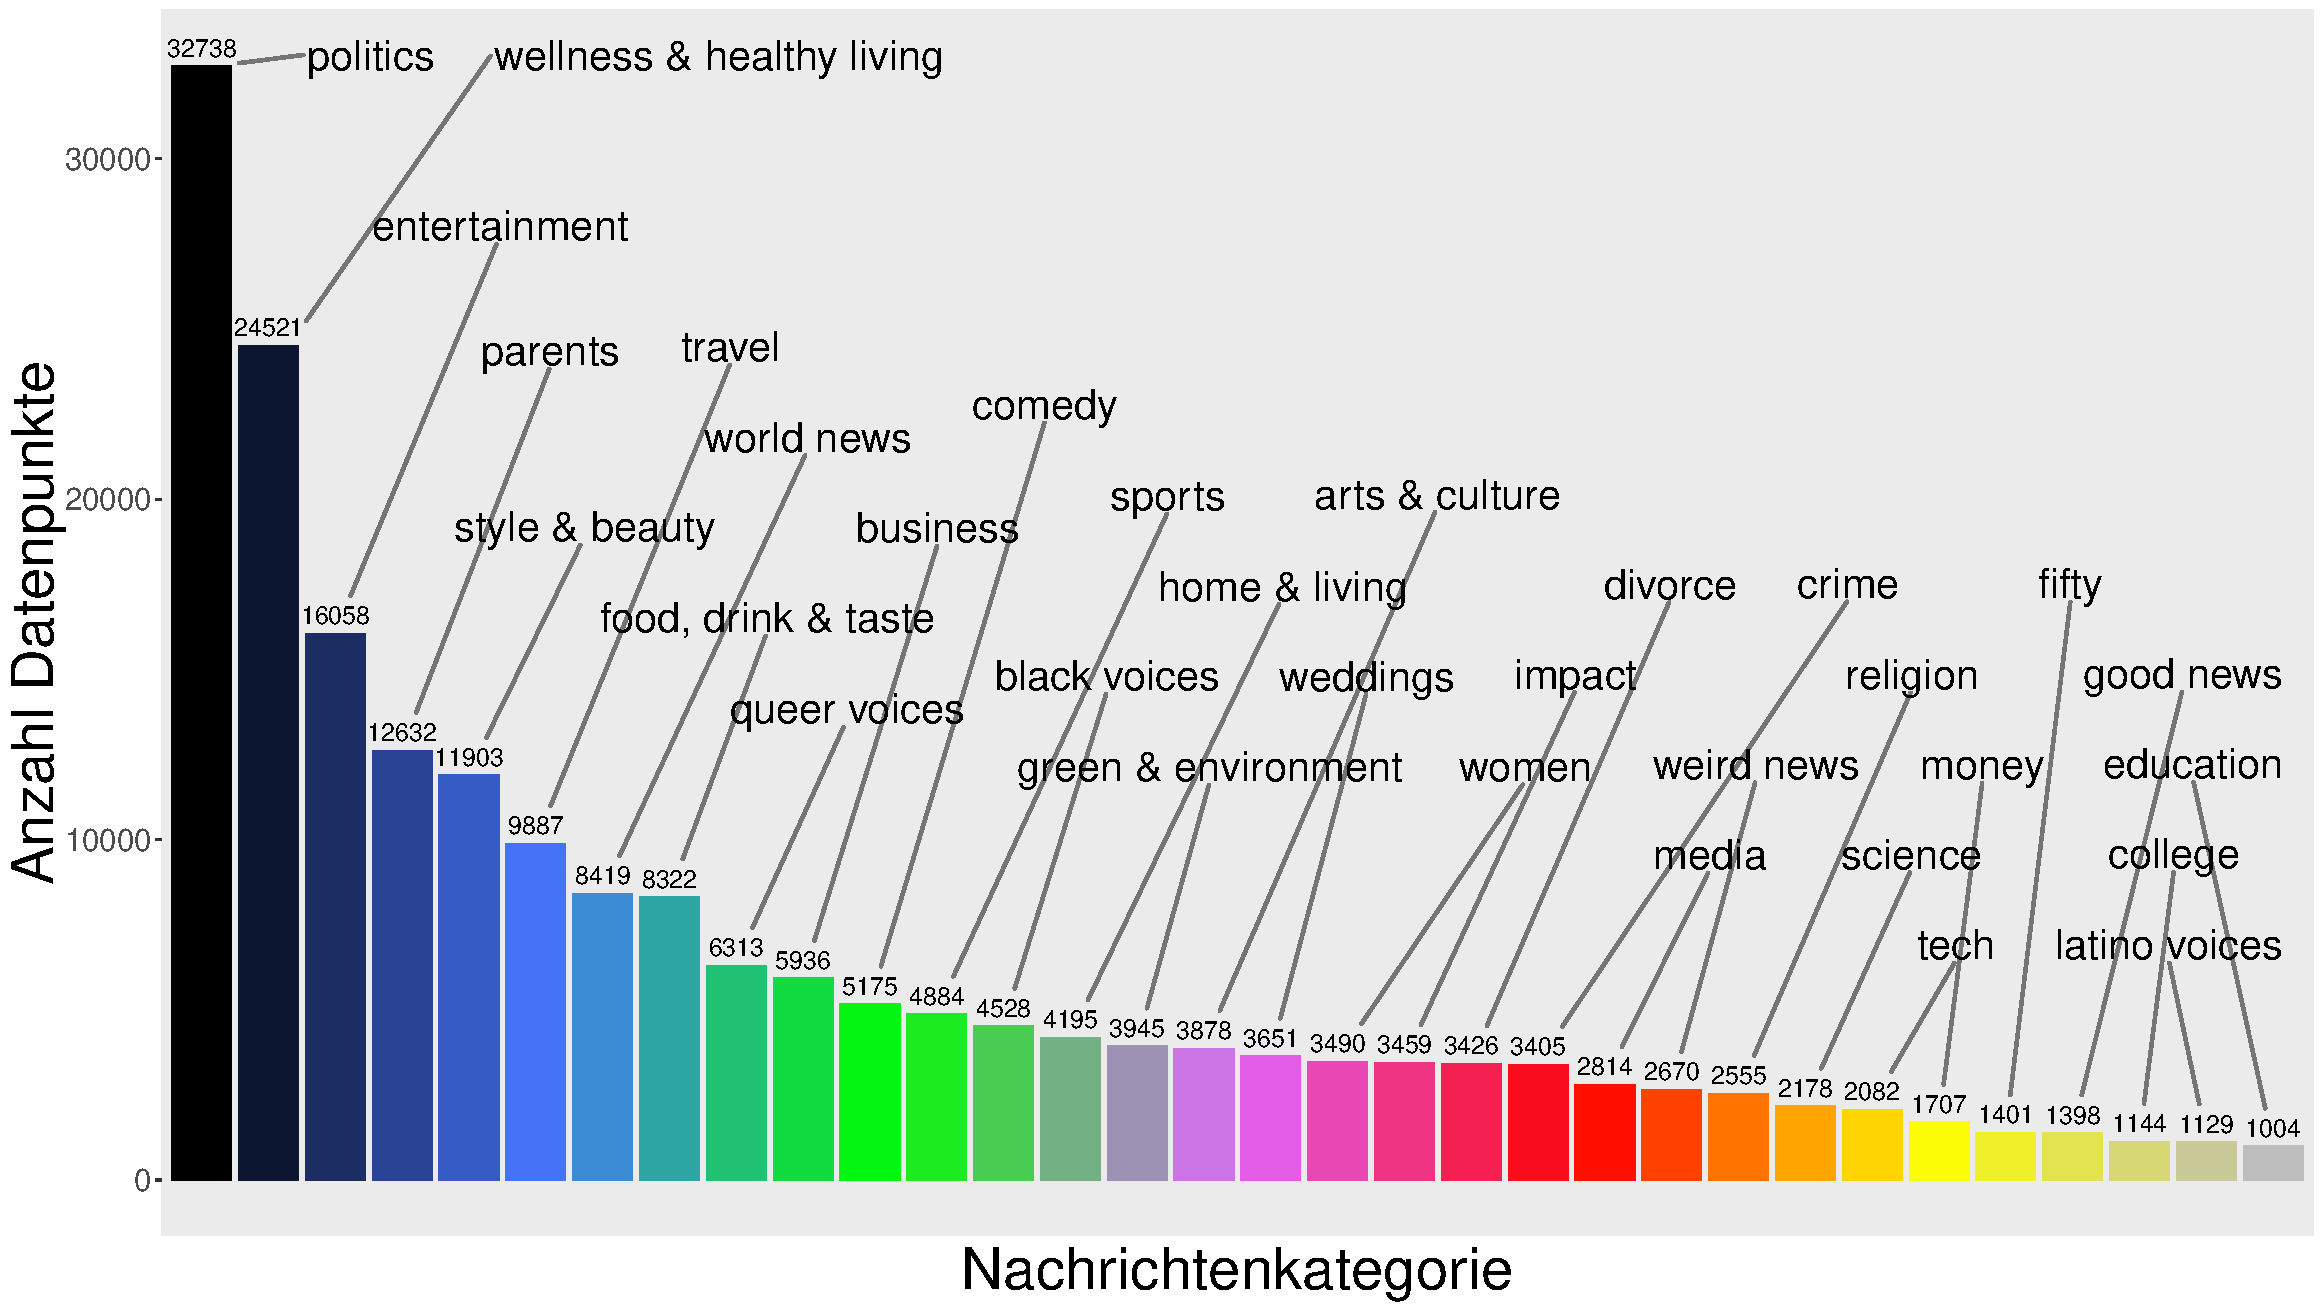
\includegraphics[width = \textwidth,  keepaspectratio]{Images/barplotCategories.pdf} 
\caption{Anzahl Datenpunkte pro Nachrichtenkategorie}
\label{abb:barplotCategories}
\end{figure}

\end{frame}


\begin{frame}

\begin{figure}[ht]
    \centering
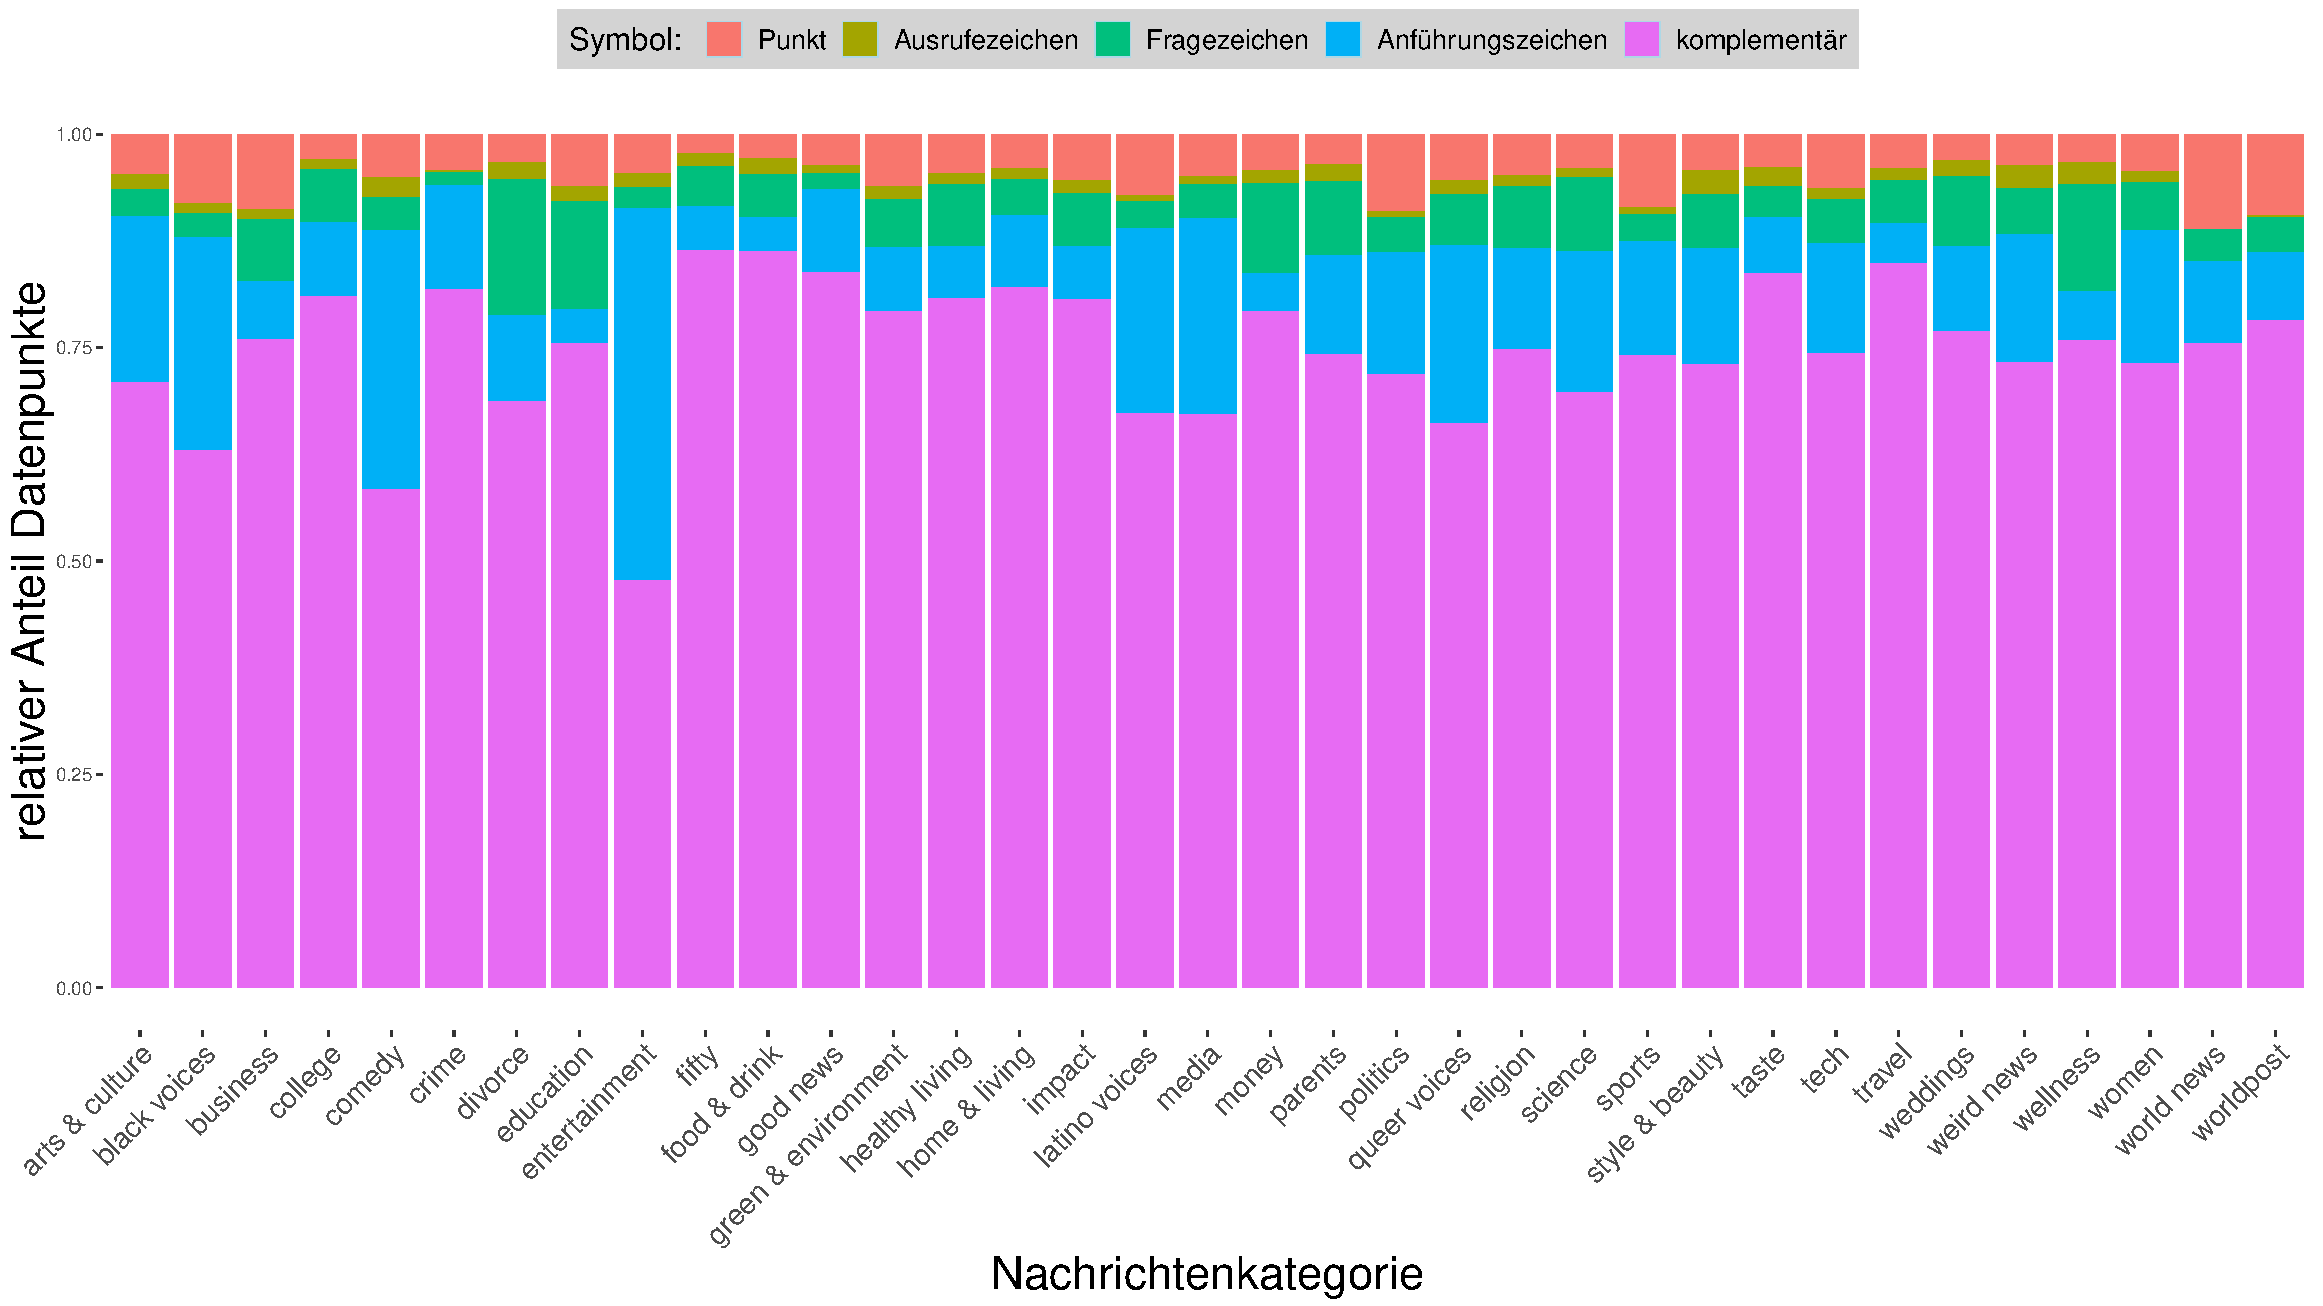
\includegraphics[width = \textwidth,  keepaspectratio]{Images/barplotSymbols.pdf} 
\caption{Relativer Anteil Datenpunkte für ausgewählte Sonderzeichen pro Kategorie. Der komplementäre Anteil ist der Anteil Datenpunkte, in dem keine der aufgeführten Sonderzeichen enthalten sind.}
\label{abb:barplotSymbols}
\end{figure}

\end{frame}


\begin{frame}
\begin{figure}[ht]
    \centering
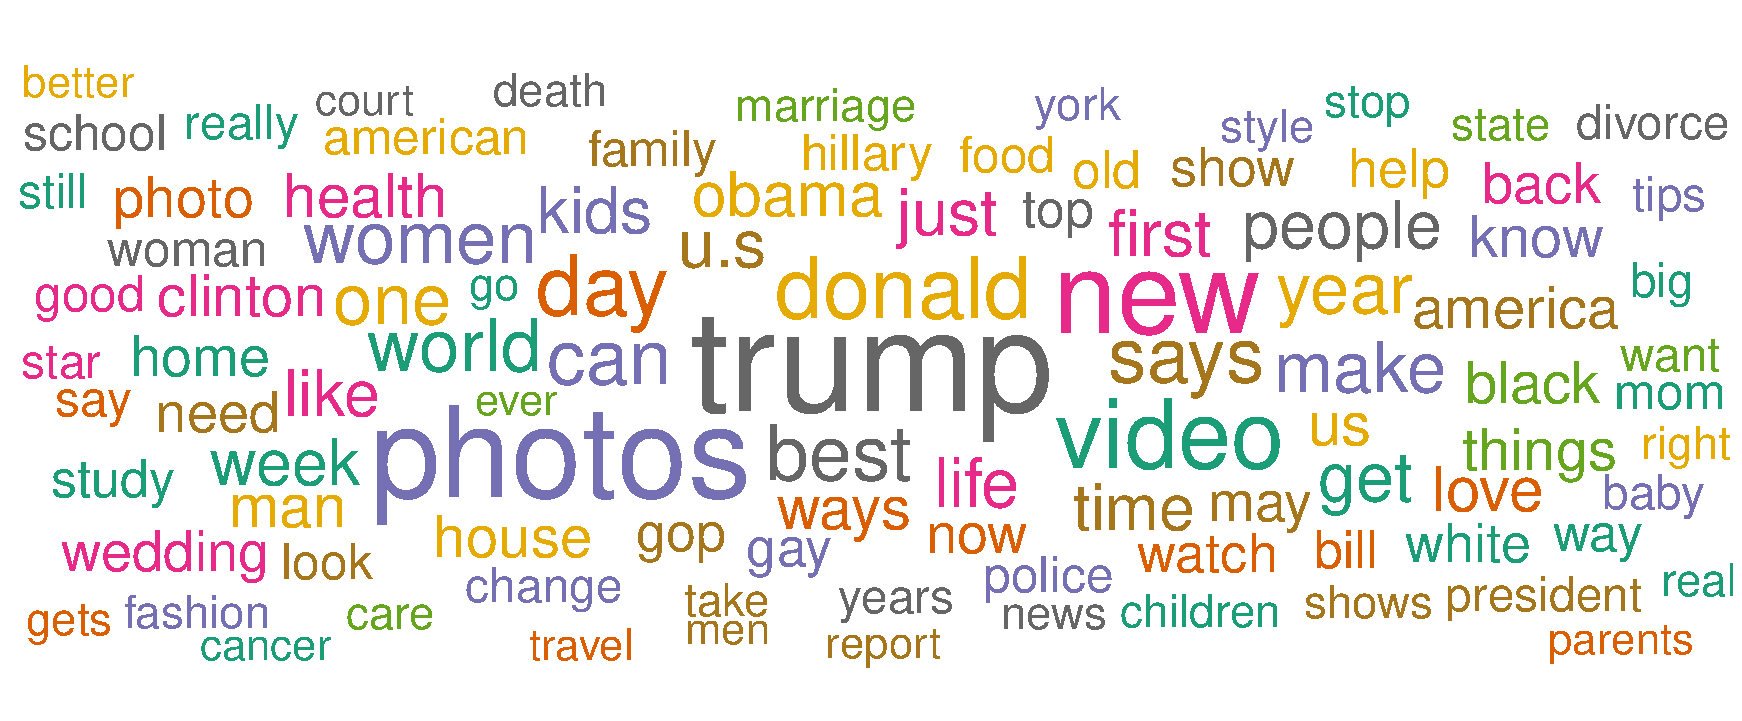
\includegraphics[width = \textwidth,  keepaspectratio]{Images/wordCloudAll.pdf} 
\caption{\textit{wordcloud} für die häufigsten 100 Wörter aller Kategorien}
\label{abb:WordcloudAll}
\end{figure}
\end{frame}


\section{Repräsentation der Wörter}

\section{Verfahren}

\section{Auswertung}

\begin{frame}{Framework}
\begin{itemize}
    \item Einteilung der \numprint{200847} Beobachtungen des gesamten Datensatzes in Trainings-, Test- und Validierungsdaten \item Testdaten $\numprint{20005}$ Beobachtungen, etwa 10 Prozent (Erwartungsgemäß $100$ in der kleinsten Kategorie)
    \item Von den $90$ Prozent der Daten, Stichprobe von $10$ Prozent gezogen ($9$ Prozent der gesamten Daten). $\numprint{18084}$ Beobachtungen
    \item Davon $80$ Prozent Trainingsdaten der Vorauswahl ($\numprint{14467}$ Datenpunkte) und $20$ Prozent  Validierungsdaten der Vorauswahl ($\numprint{3617}$ Datenpunkte)
    \item Tuning und Struktur der Netze auf Validierungsdaten
\end{itemize}{}
\end{frame}{}

\begin{frame}
\begin{figure}[ht]
    \centering
\includegraphics[width = \textwidth,  keepaspectratio]{Images/FinalSelectionAccByClass.pdf} 
\caption{}
\label{abb:AccByClass}
\end{figure}
\end{frame}

\begin{frame}
\begin{figure}[ht]
    \centering
\includegraphics[width = \textwidth,  keepaspectratio]{Images/FinalSelectionCompareProbVsAcc.pdf} 
\caption{}
\label{abb:CompareProbVsAcc}
\end{figure}
\end{frame}




\section{Fazit und Ausblick}



\end{document}